
The Exact Motif Search - Generate and Test algorithm for the planted motif search problem, first developed by Nabos \cite{nabos2015dissertation}, is composed of two main phases, the Generate phase and the Test phase. The Generate phase takes the first $n'$ number of string sequences in the dataset and generates the set $d$-neighborhood one sequence at a time then intersects it. This accumulates and outputs the set of candidate motifs $\mathcal{C}$ and is composed of $l$-mers that have at least one $d$-neighbor in each of the first $n'$ sequences. The Test phase evaluates each candidate motif $c \in C$ by comparing $c$ if it has at least one $d$-neighbor in each of the remaining $n - n'$ string sequences. \newline

\noindent These phases are formally defined below:
% show the formal definition of EMS-GT algorithm steps
\begin{enumerate} [label={\em (\alph*)}]

	\item {Generate phase} \newline
	This phase operates on the first $n'$ sequences. The intersection of the $d$-neighborhood of each sequence will result to the set of candidate motifs $C$.

	\begin{equation}
		C = \mathcal{N}(S_{1}, d) \cap \mathcal{N}(S_{2}, d) \cap...\cap \mathcal{N}(S_{n'}, d).
	\end{equation} \newline

	\item {Test phase}\newline
	Each candidate motif in $C$ will be evaluated if it appears in all of the remaining $n - n'$ string sequences. If a candidate motif pass the test, it is then included in the set of motifs $M$. 

\end{enumerate}

% 
The Exact Motif Search - Generate and Test algorithm for the planted motif search problem, first developed by Nabos \cite{nabos2015dissertation}, is composed of main two phases, the Generate phase and the Test phase. The Generate phase takes the first $n'$ number of string sequences in the dataset and generates the set $d$-neighborhood one sequence at a time then intersects it. This accumulates and outputs the set of candidate motifs $\mathcal{C}$ and is composed of $l$-mers that have at least one $d$-neighbor in each of the first $n'$ sequences. The Test phase evaluates each candidate motif $c \in C$ by comparing $c$ if it has at least one $d$-neighbor in each of the remaining $n - n'$ string sequences. \newline

\noindent These phases are formally defined below:
% show the formal definition of EMS-GT algorithm steps
\begin{enumerate} [label={\em (\alph*)}]

	\item {Generate phase} \newline
	This phase operates on the first $n'$ sequences. The intersection of the $d$-neighborhood of each sequence will result to the set of candidate motifs $C$.\newline

	\begin{equation}
		C = \mathcal{N}(S_{1}, d) \cap \mathcal{N}(S_{2}, d) \cap...\cap \mathcal{N}(S_{n'}, d).
	\end{equation} 

	\item {Test phase}\newline
	Each candidate motif in $C$ will be evaluated if it appears in all of the remaining $n - n'$ string sequences. If a candidate motif pass the test, it is then included in the set of motifs $M$. 

\end{enumerate}

% 
The Exact Motif Search - Generate and Test algorithm for the planted motif search problem, first developed by Nabos \cite{nabos2015dissertation}, is composed of main two phases, the Generate phase and the Test phase. The Generate phase takes the first $n'$ number of string sequences in the dataset and generates the set $d$-neighborhood one sequence at a time then intersects it. This accumulates and outputs the set of candidate motifs $\mathcal{C}$ and is composed of $l$-mers that have at least one $d$-neighbor in each of the first $n'$ sequences. The Test phase evaluates each candidate motif $c \in C$ by comparing $c$ if it has at least one $d$-neighbor in each of the remaining $n - n'$ string sequences. \newline

\noindent These phases are formally defined below:
% show the formal definition of EMS-GT algorithm steps
\begin{enumerate} [label={\em (\alph*)}]

	\item {Generate phase} \newline
	This phase operates on the first $n'$ sequences. The intersection of the $d$-neighborhood of each sequence will result to the set of candidate motifs $C$.\newline

	\begin{equation}
		C = \mathcal{N}(S_{1}, d) \cap \mathcal{N}(S_{2}, d) \cap...\cap \mathcal{N}(S_{n'}, d).
	\end{equation} 

	\item {Test phase}\newline
	Each candidate motif in $C$ will be evaluated if it appears in all of the remaining $n - n'$ string sequences. If a candidate motif pass the test, it is then included in the set of motifs $M$. 

\end{enumerate}

% 
The Exact Motif Search - Generate and Test algorithm for the planted motif search problem, first developed by Nabos \cite{nabos2015dissertation}, is composed of main two phases, the Generate phase and the Test phase. The Generate phase takes the first $n'$ number of string sequences in the dataset and generates the set $d$-neighborhood one sequence at a time then intersects it. This accumulates and outputs the set of candidate motifs $\mathcal{C}$ and is composed of $l$-mers that have at least one $d$-neighbor in each of the first $n'$ sequences. The Test phase evaluates each candidate motif $c \in C$ by comparing $c$ if it has at least one $d$-neighbor in each of the remaining $n - n'$ string sequences. \newline

\noindent These phases are formally defined below:
% show the formal definition of EMS-GT algorithm steps
\begin{enumerate} [label={\em (\alph*)}]

	\item {Generate phase} \newline
	This phase operates on the first $n'$ sequences. The intersection of the $d$-neighborhood of each sequence will result to the set of candidate motifs $C$.\newline

	\begin{equation}
		C = \mathcal{N}(S_{1}, d) \cap \mathcal{N}(S_{2}, d) \cap...\cap \mathcal{N}(S_{n'}, d).
	\end{equation} 

	\item {Test phase}\newline
	Each candidate motif in $C$ will be evaluated if it appears in all of the remaining $n - n'$ string sequences. If a candidate motif pass the test, it is then included in the set of motifs $M$. 

\end{enumerate}

% \input{contents/pseudocode/ems-gt}

% \input{contents/pseudocode/recursive-neighborhood-gen}

Data structures and the how an algorithm deals with the data commonly drive the performance of an algorithm. The EMS-GT algorithm uses a compressed bit-flag array for fast candidate motif elimination. Some key techniques that EMS-GT uses are defined in this section.

	\subsubsection{Integer mapping of $l$-mers}
	EMS-GT converts $l$-mers into its corresponding integer values. To achieve this, each character in the $l$-mer is translated using 2 bits (a=00, c=01, g=10, t=11). \newline
		{\small Ex.	\texttt{actg} maps to \texttt{00011110} and has an integer value of 30} 

	\subsubsection{Bit-based set representation and l-mer enumeration} 
	The EMS-GT maintains a $4^l$ array for enumerating all the possible $l$-mer values. The $l$-mer's integer value is used as the index value for the array. It uses the value of 1 if the $l$-mer is a member of the set, else it sets the value to 0.

	\subsubsection{Bit-array compression}
	To efficiently store these $l$-mers and save memory space, EMS-GT implements an approach that compresses the search space array using integer value bit flags. Instead of one $l$-mer per index value, the implementation can flag up to 32 $l$-mers (since we are using 32-bit integers) per index value. The explanation on how the algorithm accesses the bit flag is defined below: \newline

		{\small Ex. \texttt{gacgt} maps to \texttt{1000011011} = 539 in decimal.\newline
			\hspace*{64pt} \emph{bit position} = 539 mod 32 = 27;\newline
			\hspace*{64pt} \emph{array index}  = 539 / 32 = 16;\newline
			\hspace*{64pt} The bit flag for \texttt{gacgt} is in the 27$^{th}$ least significant bit\newline
			\hspace*{64pt} of the integer at array index 16.}

	\input{contents/00_figure/search_space}

	\subsubsection{XOR-based Hamming distance computation}
	The mapping of an $l$-mer to its integer value has an additional advantage in computing for mismatch positions. Applying the boolean operator exclusive-or (XOR) between two integer values will return another integer value that contains nonzero value for mismatch position. Counting this nonzero positions result to the hamming distance value. An example of this computation is shown below: \newline

	{\small Ex.	\texttt{aacgt} maps to \texttt{0000011011} \newline
		\vspace*{2pt}\hspace*{53pt} \underline{\texttt{tacgc} maps to \texttt{1100011001}} \newline
		\hspace*{55pt}	XOR produces \texttt{\uline{11}000000\uline{10}} = 2 mismatches.} \newline
		\hspace*{53pt} (Note, the mismatches are counted per pair)


	\subsubsection{Recursive neighborhood generation}
	The Generate step of the algorithm produces the $d$-neighborhood of a string sequence by generating the $d$-neighborhood of all $l$-mers in that sequence. Our implementation of EMS-GT uses a recursive approach for generating the $d$-neighborhood of an $l$-mer. The recursive generation can be visualized by a tree $\mathcal{T}(x)$ of height $d$ that is generated in depth-first manner. Each node is a tuple of $(w, p)$ where $w$ is an $l$-mer and $p$ corresponds to a position in the $l$-mer $0 \leq p \leq l$. At a given node $(w, p)$ and $p \neq l$, three children nodes are generated where each node is variant of $w$ that has a different character in $p + 1$ position. The root node is $(x, 0)$ and any $l$-mer in nodes at depth $t$ has a hamming distance of $t$ from the $l$-mer $x$. Given this, the expected size of $N(x, d)$ can be computed using the equation: \newline
	\begin{equation}
		|N(x,d)| = \sum_{i=0}^d \binom{l}{i} 3^{i}
	\end{equation}

	\input{contents/00_figure/neighborhood_generation}

	\subsubsection{Block-based optimization for neighborhood generation}
	The way EMS-GT represents the $d$-neighborhood $N_x$ of $l$-mer $x$ opens up a new way to improve the generation of neighborhood. $N_x$ is represented by a compresed $4^l$ bit flags array, where value of 1 corresponds to set membership, 0 if otherwise.  A previous study by Sia \cite{sia2015} improved the runtime performance in generating $N_x$. If $N_x$ is partitioned into blocks of $4^k$ bits each, where $k < l$, each block will conform into ($k$ + 2) bit patterns. By pre-computing these patterns, the algorithm can build the $N_x$ by blocks of bits instead of one bit at a time.

	\input{contents/00_figure/bit-patterns}

	The algorithm divides the $l$-mer $x$ into its $(l - k)$-length prefix $y$ and suffix $z$ of length $k$. With the block patterns of $4^k$ $l$-mers generated, the algorithm recursively generates all possible prefix of $x$. For each prefix $y'$ generated, the algorithm applies the corresponding block pattern in $N_x$ based on $z$ and the remaining number of allowed mutations $d'$, where $d' = d - d_H(y, y')$. Specifically, EMS-GT builds the $\mathcal{N}_S$ using these steps:

	\begin{enumerate}
		\item Initialize $\mathcal{N}_S$ as an array of $4^l$ bits set to zero, and select a value for $k$.

		\item Pre-generate {\em Pattern}( $z$, $d_z$ ) for all $z \in \Sigma^k$ and all $d_z \in \{1,...,k-1\}$ to serve as bit masks for blocks. Note that block patterns for $d_z=0$ (one bit set) and $d_z=k$ (all bits set) will not require bit masks.

		\item For each $l$-mer $x = yz$ in sequence $S$: take each neighbor $y'$ of $y$, find the block in $\mathcal{N}_S$ whose prefix is $y'$, and compute the allowable suffix mismatches $d_z = d - d_H(y,y')$ within this block. Then,

			\begin{enumerate}
				\item if $d_z = 0$, set the bit at position $z$ in the block;
				\item if $d_z \geq k$, set all bits in the block to 1;
				\item otherwise, mask {\em Pattern}( $z$, $d_z$ ) onto the block.
			\end{enumerate}
	\end{enumerate}

	Choosing the optimum value for $k$ is important in this speedup technique. The $k$ value determines the runtime complexity of this technique since $k$ value determines the size of the block patterns. When $k$ value is higher, there are fewer prefix to generate recursively but each block bits setting is large. When $k$ value is lower, block bits setting is small but the algorithm has to recursively generate a larger number of prefix value of $l$-mer $x$. The optimum $k$ value used in the study is 5.

	\input{contents/00_pseudocodes/block-pattern-generation}

	% Elaborate and include results
	% Mention its competitiveness and a bit of introduction on possible areas of improvement 
	EMS-GT with this speedup technique has proven its competitiveness against algorithms qPMSPrune, qPMS7, PMS8 and qPMS9. Previous experimentations showed that EMS-GT with this speedup technique outperforms PMS8 in challenge instances (9, 2), (11, 3), (13, 4), (15, 5) and (17, 6). Compared to qPMS9, the improved EMS-GT is faster on all challenge instances mentioned except (17, 6). This study aims to outperform qPMS9 for challenges up to (17, 6).

	\input{contents/00_figure/sia-bar-results}

% \begin{figure}[b]
	\noindent \hspace*{6pt}{\bf Algorithm 2} \textsc{Generate Neighborhood}
	\begin{algorithmic}[1]
		\label{alg:recursive-nbr-gen}
		\Require DNA sequence $S$, motif length $l$, mismatches $d$
		\Ensure bit-array $\mathcal{N}$ representing $\mathcal{N}(S,d)$ \vspace*{6pt}
		% \For{$i \leftarrow$ 1 to $4^{l}$}
		\State $\mathcal{N}[i] \leftarrow 0,\ \ \forall i < 4^{l}$ 
		% \EndFor
		\For{each $l$-mer $x$ in $S$}
			\State \textsc{AddNeighbors}($x$, 0, $d$) \hspace*{9pt}\Comment{recursive procedure}
		\EndFor
		\State \Comment{make $d$ changes in $l$-mer $x$, from position $s$ onward}
		\Procedure{AddNeighbors}{$x$, $s$, $d$}
			\For{$i \leftarrow s$ to $l$}
				\State $\Sigma \leftarrow$ \{\texttt{a}, \texttt{g}, \texttt{c}, \texttt{t}\} $- x_{i}$ \hspace*{6pt}\Comment{$i^{th}$ character in $x$}
				\For{$j \leftarrow 1$ to $|\Sigma|$}
					\State $neighbor \leftarrow\ ${\em\small concatenate}$(x_{1...i-1},\Sigma_{j},x_{i+1...l})$
					\State $\mathcal{N}[neighbor] \leftarrow 1$
					\If{$d > 1$ and $i < l$}
						\State \textsc{AddNeighbors}($neighbor$, $i+1$, $d-1$)
					\EndIf
				\EndFor
			\EndFor
		\EndProcedure
		\State\Return $\mathcal{N}$
	\end{algorithmic}
\end{figure}

Data structures and the how an algorithm deals with the data commonly drive the performance of an algorithm. The EMS-GT algorithm uses a compressed bit-flag array for fast candidate motif elimination. Some key techniques that EMS-GT uses are defined in this section.

	\subsubsection{Integer mapping of $l$-mers}
	EMS-GT converts $l$-mers into its corresponding integer values. To achieve this, each character in the $l$-mer is translated using 2 bits (a=00, c=01, g=10, t=11). \newline
		{\small Ex.	\texttt{actg} maps to \texttt{00011110} and has an integer value of 30} 

	\subsubsection{Bit-based set representation and l-mer enumeration} 
	The EMS-GT maintains a $4^l$ array for enumerating all the possible $l$-mer values. The $l$-mer's integer value is used as the index value for the array. It uses the value of 1 if the $l$-mer is a member of the set, else it sets the value to 0.

	\subsubsection{Bit-array compression}
	To efficiently store these $l$-mers and save memory space, EMS-GT implements an approach that compresses the search space array using integer value bit flags. Instead of one $l$-mer per index value, the implementation can flag up to 32 $l$-mers (since we are using 32-bit integers) per index value. The explanation on how the algorithm accesses the bit flag is defined below: \newline

		{\small Ex. \texttt{gacgt} maps to \texttt{1000011011} = 539 in decimal.\newline
			\hspace*{64pt} \emph{bit position} = 539 mod 32 = 27;\newline
			\hspace*{64pt} \emph{array index}  = 539 / 32 = 16;\newline
			\hspace*{64pt} The bit flag for \texttt{gacgt} is in the 27$^{th}$ least significant bit\newline
			\hspace*{64pt} of the integer at array index 16.}

	\begin{figure}[h]
	\centering
	\label{fig:search_space}
	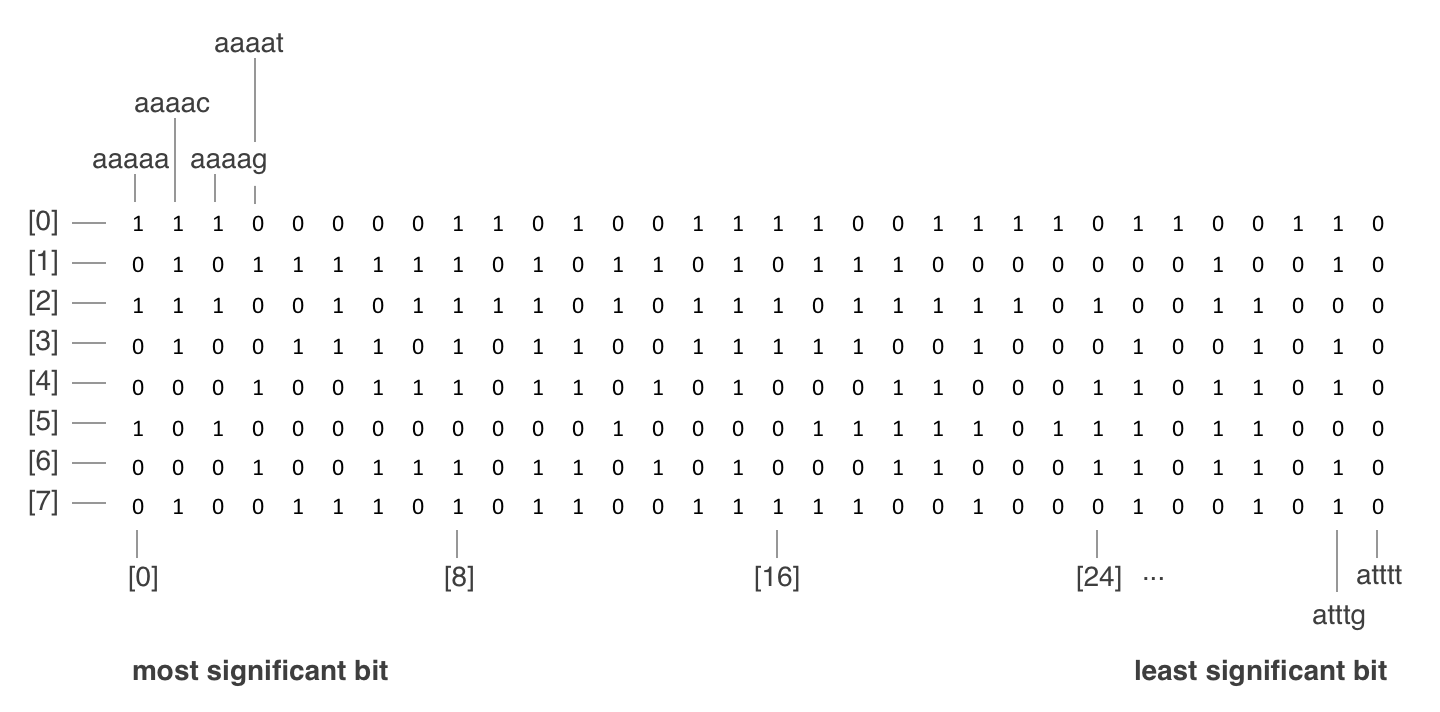
\includegraphics[width=5in]{contents/00_images/search_space}\vspace*{5pt}
	\caption{First 8 rows of the $4^{5}$ search space with random flag values.}
\end{figure}

	\subsubsection{XOR-based Hamming distance computation}
	The mapping of an $l$-mer to its integer value has an additional advantage in computing for mismatch positions. Applying the boolean operator exclusive-or (XOR) between two integer values will return another integer value that contains nonzero value for mismatch position. Counting this nonzero positions result to the hamming distance value. An example of this computation is shown below: \newline

	{\small Ex.	\texttt{aacgt} maps to \texttt{0000011011} \newline
		\vspace*{2pt}\hspace*{53pt} \underline{\texttt{tacgc} maps to \texttt{1100011001}} \newline
		\hspace*{55pt}	XOR produces \texttt{\uline{11}000000\uline{10}} = 2 mismatches.} \newline
		\hspace*{53pt} (Note, the mismatches are counted per pair)


	\subsubsection{Recursive neighborhood generation}
	The Generate step of the algorithm produces the $d$-neighborhood of a string sequence by generating the $d$-neighborhood of all $l$-mers in that sequence. Our implementation of EMS-GT uses a recursive approach for generating the $d$-neighborhood of an $l$-mer. The recursive generation can be visualized by a tree $\mathcal{T}(x)$ of height $d$ that is generated in depth-first manner. Each node is a tuple of $(w, p)$ where $w$ is an $l$-mer and $p$ corresponds to a position in the $l$-mer $0 \leq p \leq l$. At a given node $(w, p)$ and $p \neq l$, three children nodes are generated where each node is variant of $w$ that has a different character in $p + 1$ position. The root node is $(x, 0)$ and any $l$-mer in nodes at depth $t$ has a hamming distance of $t$ from the $l$-mer $x$. Given this, the expected size of $N(x, d)$ can be computed using the equation: \newline
	\begin{equation}
		|N(x,d)| = \sum_{i=0}^d \binom{l}{i} 3^{i}
	\end{equation}

	\begin{figure}[h]
	\centering
	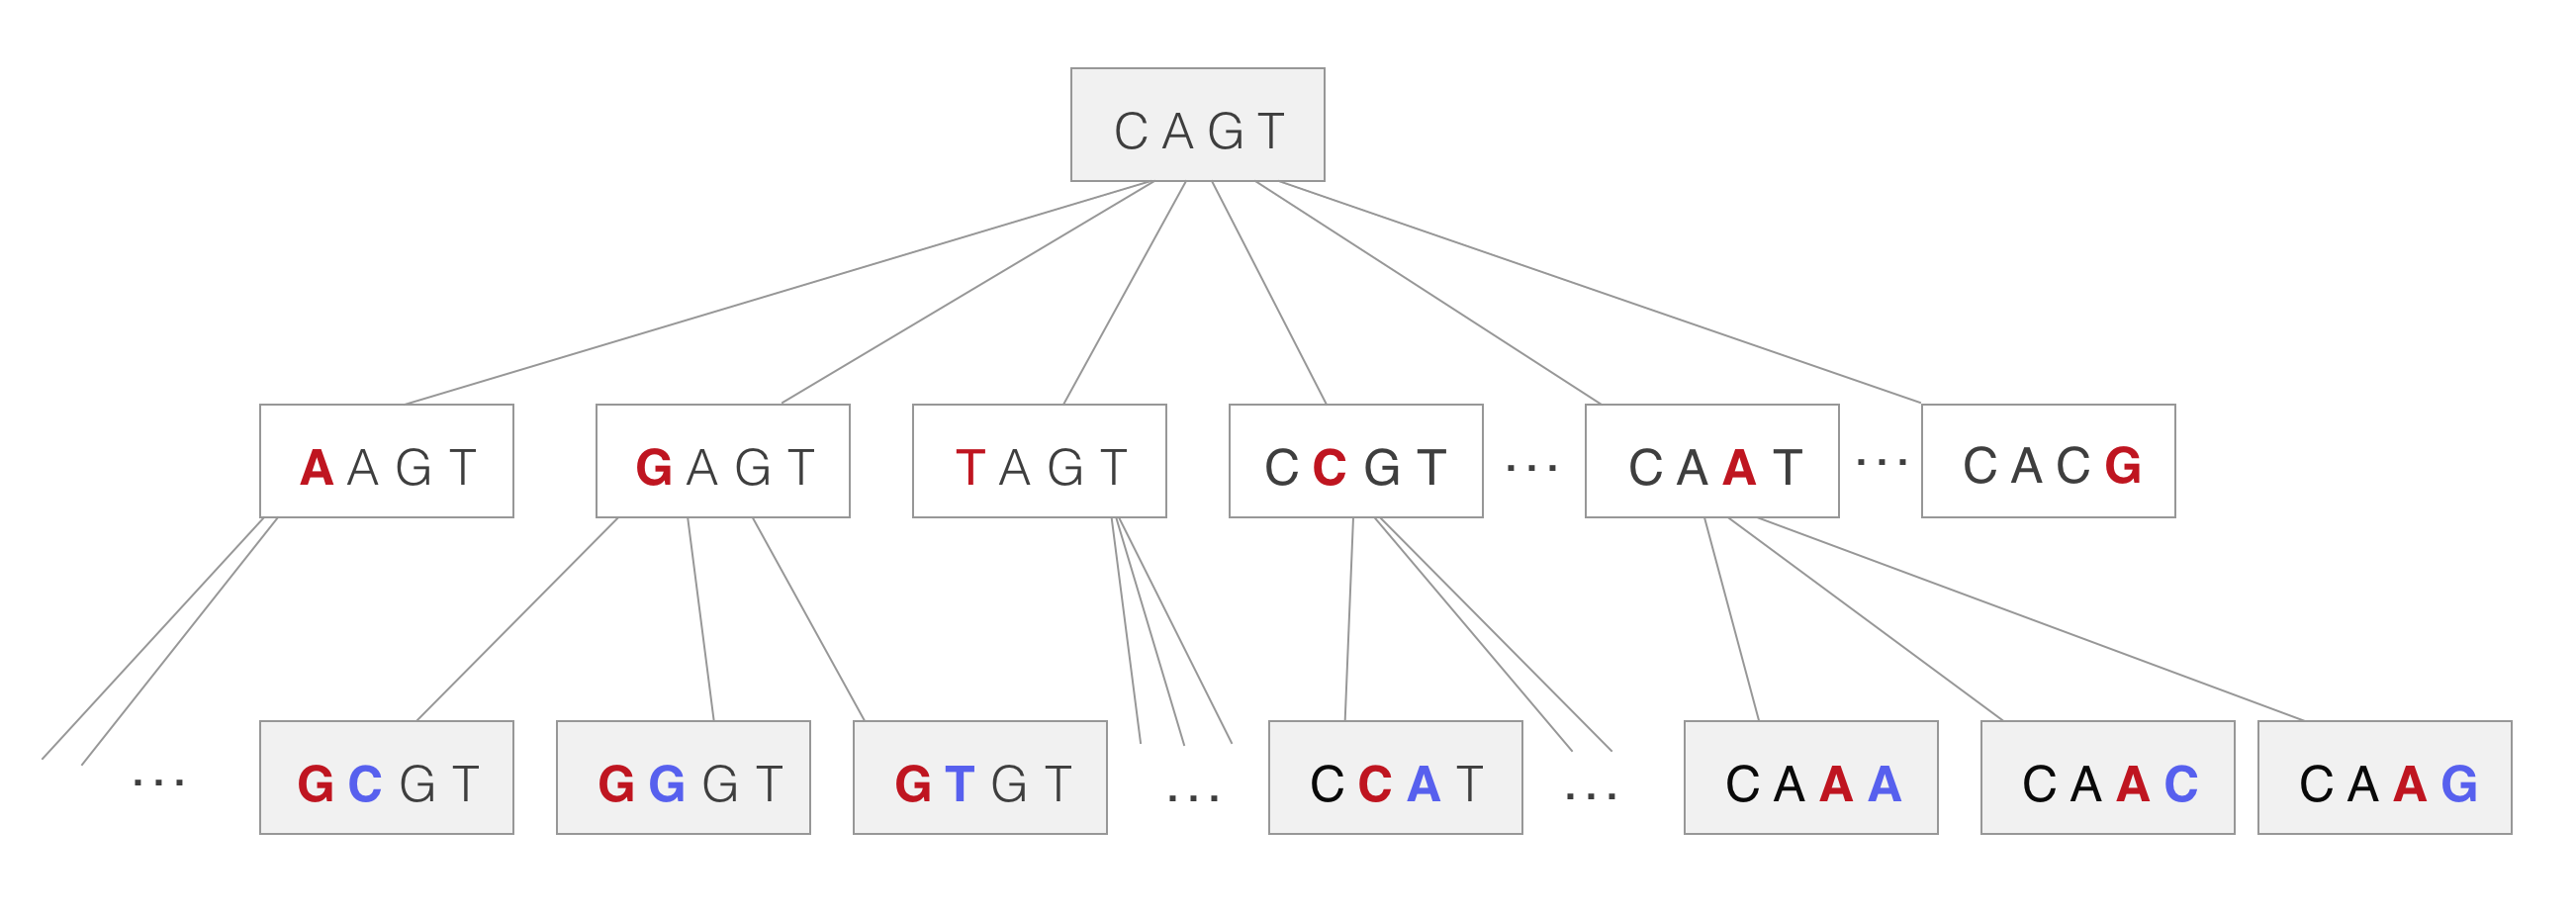
\includegraphics[width=5in]{contents/00_images/neighborhood-generation}\vspace*{5pt}
	\caption{Recursively generating the neighborhood of $l$-mer CACGT with $d = 2$}
	\label{fig:neighborhood-generation}
\end{figure}

	\subsubsection{Block-based optimization for neighborhood generation}
	The way EMS-GT represents the $d$-neighborhood $N_x$ of $l$-mer $x$ opens up a new way to improve the generation of neighborhood. $N_x$ is represented by a compresed $4^l$ bit flags array, where value of 1 corresponds to set membership, 0 if otherwise.  A previous study by Sia \cite{sia2015} improved the runtime performance in generating $N_x$. If $N_x$ is partitioned into blocks of $4^k$ bits each, where $k < l$, each block will conform into ($k$ + 2) bit patterns. By pre-computing these patterns, the algorithm can build the $N_x$ by blocks of bits instead of one bit at a time.

	\begin{figure}[h]
	\centering
	
\includegraphics[width=2.5in]{contents/00_images/0-1}\vspace*{5pt}
	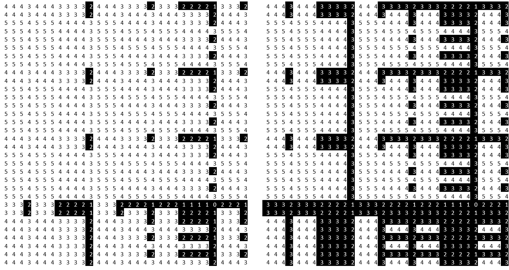
\includegraphics[width=2.5in]{contents/00_images/2-3}\vspace*{5pt}
	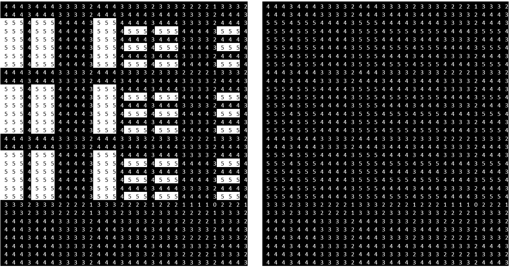
\includegraphics[width=2.5in]{contents/00_images/4-5}
	
	\caption{Bit patterns followed by blocks of size $4^{5}=32\times32$ in the bit-based representation of $\mathcal{N}(\texttt{acgtacgtacgt},5)$. Black signifies a 1. There are $(5+2)=7$ possible patterns---the empty pattern (all 0s) is not shown. Images from \cite{sia2015}}
	\label{fig:bit_patterns}
\end{figure}

	The algorithm divides the $l$-mer $x$ into its $(l - k)$-length prefix $y$ and suffix $z$ of length $k$. With the block patterns of $4^k$ $l$-mers generated, the algorithm recursively generates all possible prefix of $x$. For each prefix $y'$ generated, the algorithm applies the corresponding block pattern in $N_x$ based on $z$ and the remaining number of allowed mutations $d'$, where $d' = d - d_H(y, y')$. Specifically, EMS-GT builds the $\mathcal{N}_S$ using these steps:

	\begin{enumerate}
		\item Initialize $\mathcal{N}_S$ as an array of $4^l$ bits set to zero, and select a value for $k$.

		\item Pre-generate {\em Pattern}( $z$, $d_z$ ) for all $z \in \Sigma^k$ and all $d_z \in \{1,...,k-1\}$ to serve as bit masks for blocks. Note that block patterns for $d_z=0$ (one bit set) and $d_z=k$ (all bits set) will not require bit masks.

		\item For each $l$-mer $x = yz$ in sequence $S$: take each neighbor $y'$ of $y$, find the block in $\mathcal{N}_S$ whose prefix is $y'$, and compute the allowable suffix mismatches $d_z = d - d_H(y,y')$ within this block. Then,

			\begin{enumerate}
				\item if $d_z = 0$, set the bit at position $z$ in the block;
				\item if $d_z \geq k$, set all bits in the block to 1;
				\item otherwise, mask {\em Pattern}( $z$, $d_z$ ) onto the block.
			\end{enumerate}
	\end{enumerate}

	Choosing the optimum value for $k$ is important in this speedup technique. The $k$ value determines the runtime complexity of this technique since $k$ value determines the size of the block patterns. When $k$ value is higher, there are fewer prefix to generate recursively but each block bits setting is large. When $k$ value is lower, block bits setting is small but the algorithm has to recursively generate a larger number of prefix value of $l$-mer $x$. The optimum $k$ value used in the study is 5.

	
% {\setstretch{1.0} % Algorithm 4.1. Block Pattern Generation
\begin{figure}[h]
	\noindent \hspace*{6pt}{\bf Algorithm 2.1}
	\textsc{Block Pattern Generation}\small
	\begin{algorithmic}[1]\label{alg:block-pattern-gen}
		\Require block degree $k$
		\Ensure 3D bit-array $\mathcal{P}$ containing all possible non-trivial block patterns \vspace*{6pt}

		\State $\mathcal{P}[\ ][\ ][\ ] \leftarrow \{\}$ \hspace*{90pt}
		\Comment{retrieve a pattern $P$ as $\mathcal{P}[z][d - d_{y'}]$ }

		\For {$z \leftarrow 0$ to $4^k$}
		\For {$j \leftarrow 1$ to $k-1$}
		\For {$z' \leftarrow 0$ to $4^k$}
		\If{$dH(z,z') \leq j$} 
			\State $\mathcal{P}[z][j][z'] \leftarrow 1$
		\Else
			\State $\mathcal{P}[z][j][z'] \leftarrow 0$
		\EndIf\EndFor\EndFor\EndFor
		\State\Return $\mathcal{P}$
		\end{algorithmic}
\end{figure}



	% Elaborate and include results
	% Mention its competitiveness and a bit of introduction on possible areas of improvement 
	EMS-GT with this speedup technique has proven its competitiveness against algorithms qPMSPrune, qPMS7, PMS8 and qPMS9. Previous experimentations showed that EMS-GT with this speedup technique outperforms PMS8 in challenge instances (9, 2), (11, 3), (13, 4), (15, 5) and (17, 6). Compared to qPMS9, the improved EMS-GT is faster on all challenge instances mentioned except (17, 6). This study aims to outperform qPMS9 for challenges up to (17, 6).

	
\begin{figure}[ht]\label{fig:results2}
	\centering
	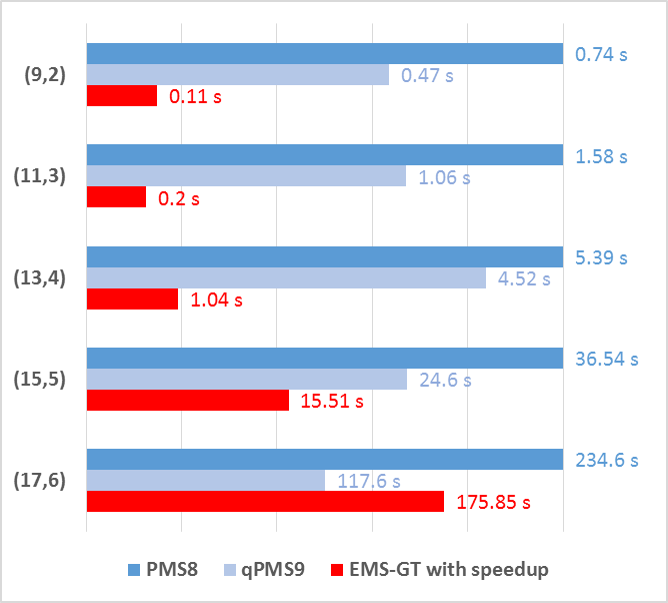
\includegraphics[width=4.0in]{contents/00_images/emsgt-with-speedup-vs-PMS,qPMS9}
	\caption{Improved EMS-GT's performance vs. PMS8 (baseline) and qPMS9. Images from \cite{sia2015}}
	\label{fig:sia-bar-results}
\end{figure}

% \begin{figure}[b]
	\noindent \hspace*{6pt}{\bf Algorithm 2} \textsc{Generate Neighborhood}
	\begin{algorithmic}[1]
		\label{alg:recursive-nbr-gen}
		\Require DNA sequence $S$, motif length $l$, mismatches $d$
		\Ensure bit-array $\mathcal{N}$ representing $\mathcal{N}(S,d)$ \vspace*{6pt}
		% \For{$i \leftarrow$ 1 to $4^{l}$}
		\State $\mathcal{N}[i] \leftarrow 0,\ \ \forall i < 4^{l}$ 
		% \EndFor
		\For{each $l$-mer $x$ in $S$}
			\State \textsc{AddNeighbors}($x$, 0, $d$) \hspace*{9pt}\Comment{recursive procedure}
		\EndFor
		\State \Comment{make $d$ changes in $l$-mer $x$, from position $s$ onward}
		\Procedure{AddNeighbors}{$x$, $s$, $d$}
			\For{$i \leftarrow s$ to $l$}
				\State $\Sigma \leftarrow$ \{\texttt{a}, \texttt{g}, \texttt{c}, \texttt{t}\} $- x_{i}$ \hspace*{6pt}\Comment{$i^{th}$ character in $x$}
				\For{$j \leftarrow 1$ to $|\Sigma|$}
					\State $neighbor \leftarrow\ ${\em\small concatenate}$(x_{1...i-1},\Sigma_{j},x_{i+1...l})$
					\State $\mathcal{N}[neighbor] \leftarrow 1$
					\If{$d > 1$ and $i < l$}
						\State \textsc{AddNeighbors}($neighbor$, $i+1$, $d-1$)
					\EndIf
				\EndFor
			\EndFor
		\EndProcedure
		\State\Return $\mathcal{N}$
	\end{algorithmic}
\end{figure}

Data structures and the how an algorithm deals with the data commonly drive the performance of an algorithm. The EMS-GT algorithm uses a compressed bit-flag array for fast candidate motif elimination. Some key techniques that EMS-GT uses are defined in this section.

	\subsubsection{Integer mapping of $l$-mers}
	EMS-GT converts $l$-mers into its corresponding integer values. To achieve this, each character in the $l$-mer is translated using 2 bits (a=00, c=01, g=10, t=11). \newline
		{\small Ex.	\texttt{actg} maps to \texttt{00011110} and has an integer value of 30} 

	\subsubsection{Bit-based set representation and l-mer enumeration} 
	The EMS-GT maintains a $4^l$ array for enumerating all the possible $l$-mer values. The $l$-mer's integer value is used as the index value for the array. It uses the value of 1 if the $l$-mer is a member of the set, else it sets the value to 0.

	\subsubsection{Bit-array compression}
	To efficiently store these $l$-mers and save memory space, EMS-GT implements an approach that compresses the search space array using integer value bit flags. Instead of one $l$-mer per index value, the implementation can flag up to 32 $l$-mers (since we are using 32-bit integers) per index value. The explanation on how the algorithm accesses the bit flag is defined below: \newline

		{\small Ex. \texttt{gacgt} maps to \texttt{1000011011} = 539 in decimal.\newline
			\hspace*{64pt} \emph{bit position} = 539 mod 32 = 27;\newline
			\hspace*{64pt} \emph{array index}  = 539 / 32 = 16;\newline
			\hspace*{64pt} The bit flag for \texttt{gacgt} is in the 27$^{th}$ least significant bit\newline
			\hspace*{64pt} of the integer at array index 16.}

	\begin{figure}[h]
	\centering
	\label{fig:search_space}
	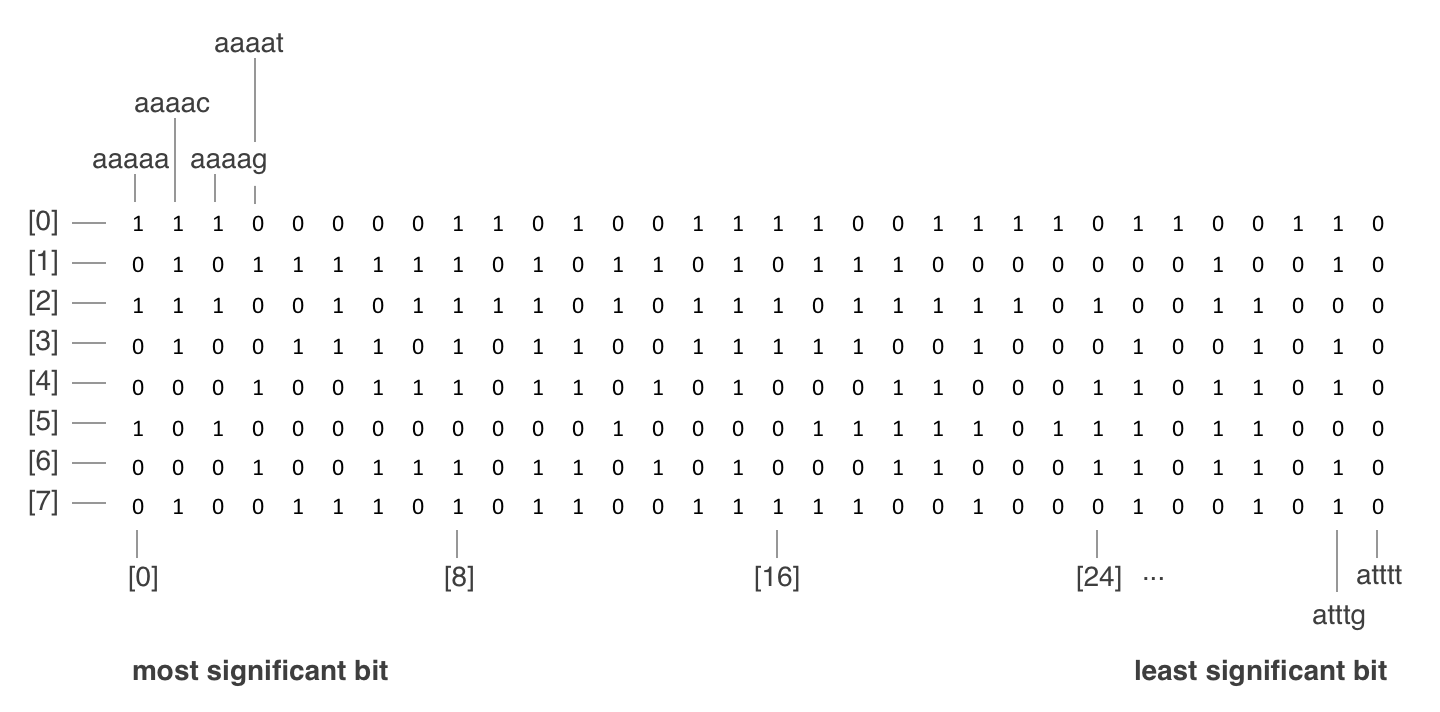
\includegraphics[width=5in]{contents/00_images/search_space}\vspace*{5pt}
	\caption{First 8 rows of the $4^{5}$ search space with random flag values.}
\end{figure}

	\subsubsection{XOR-based Hamming distance computation}
	The mapping of an $l$-mer to its integer value has an additional advantage in computing for mismatch positions. Applying the boolean operator exclusive-or (XOR) between two integer values will return another integer value that contains nonzero value for mismatch position. Counting this nonzero positions result to the hamming distance value. An example of this computation is shown below: \newline

	{\small Ex.	\texttt{aacgt} maps to \texttt{0000011011} \newline
		\vspace*{2pt}\hspace*{53pt} \underline{\texttt{tacgc} maps to \texttt{1100011001}} \newline
		\hspace*{55pt}	XOR produces \texttt{\uline{11}000000\uline{10}} = 2 mismatches.} \newline
		\hspace*{53pt} (Note, the mismatches are counted per pair)


	\subsubsection{Recursive neighborhood generation}
	The Generate step of the algorithm produces the $d$-neighborhood of a string sequence by generating the $d$-neighborhood of all $l$-mers in that sequence. Our implementation of EMS-GT uses a recursive approach for generating the $d$-neighborhood of an $l$-mer. The recursive generation can be visualized by a tree $\mathcal{T}(x)$ of height $d$ that is generated in depth-first manner. Each node is a tuple of $(w, p)$ where $w$ is an $l$-mer and $p$ corresponds to a position in the $l$-mer $0 \leq p \leq l$. At a given node $(w, p)$ and $p \neq l$, three children nodes are generated where each node is variant of $w$ that has a different character in $p + 1$ position. The root node is $(x, 0)$ and any $l$-mer in nodes at depth $t$ has a hamming distance of $t$ from the $l$-mer $x$. Given this, the expected size of $N(x, d)$ can be computed using the equation: \newline
	\begin{equation}
		|N(x,d)| = \sum_{i=0}^d \binom{l}{i} 3^{i}
	\end{equation}

	\begin{figure}[h]
	\centering
	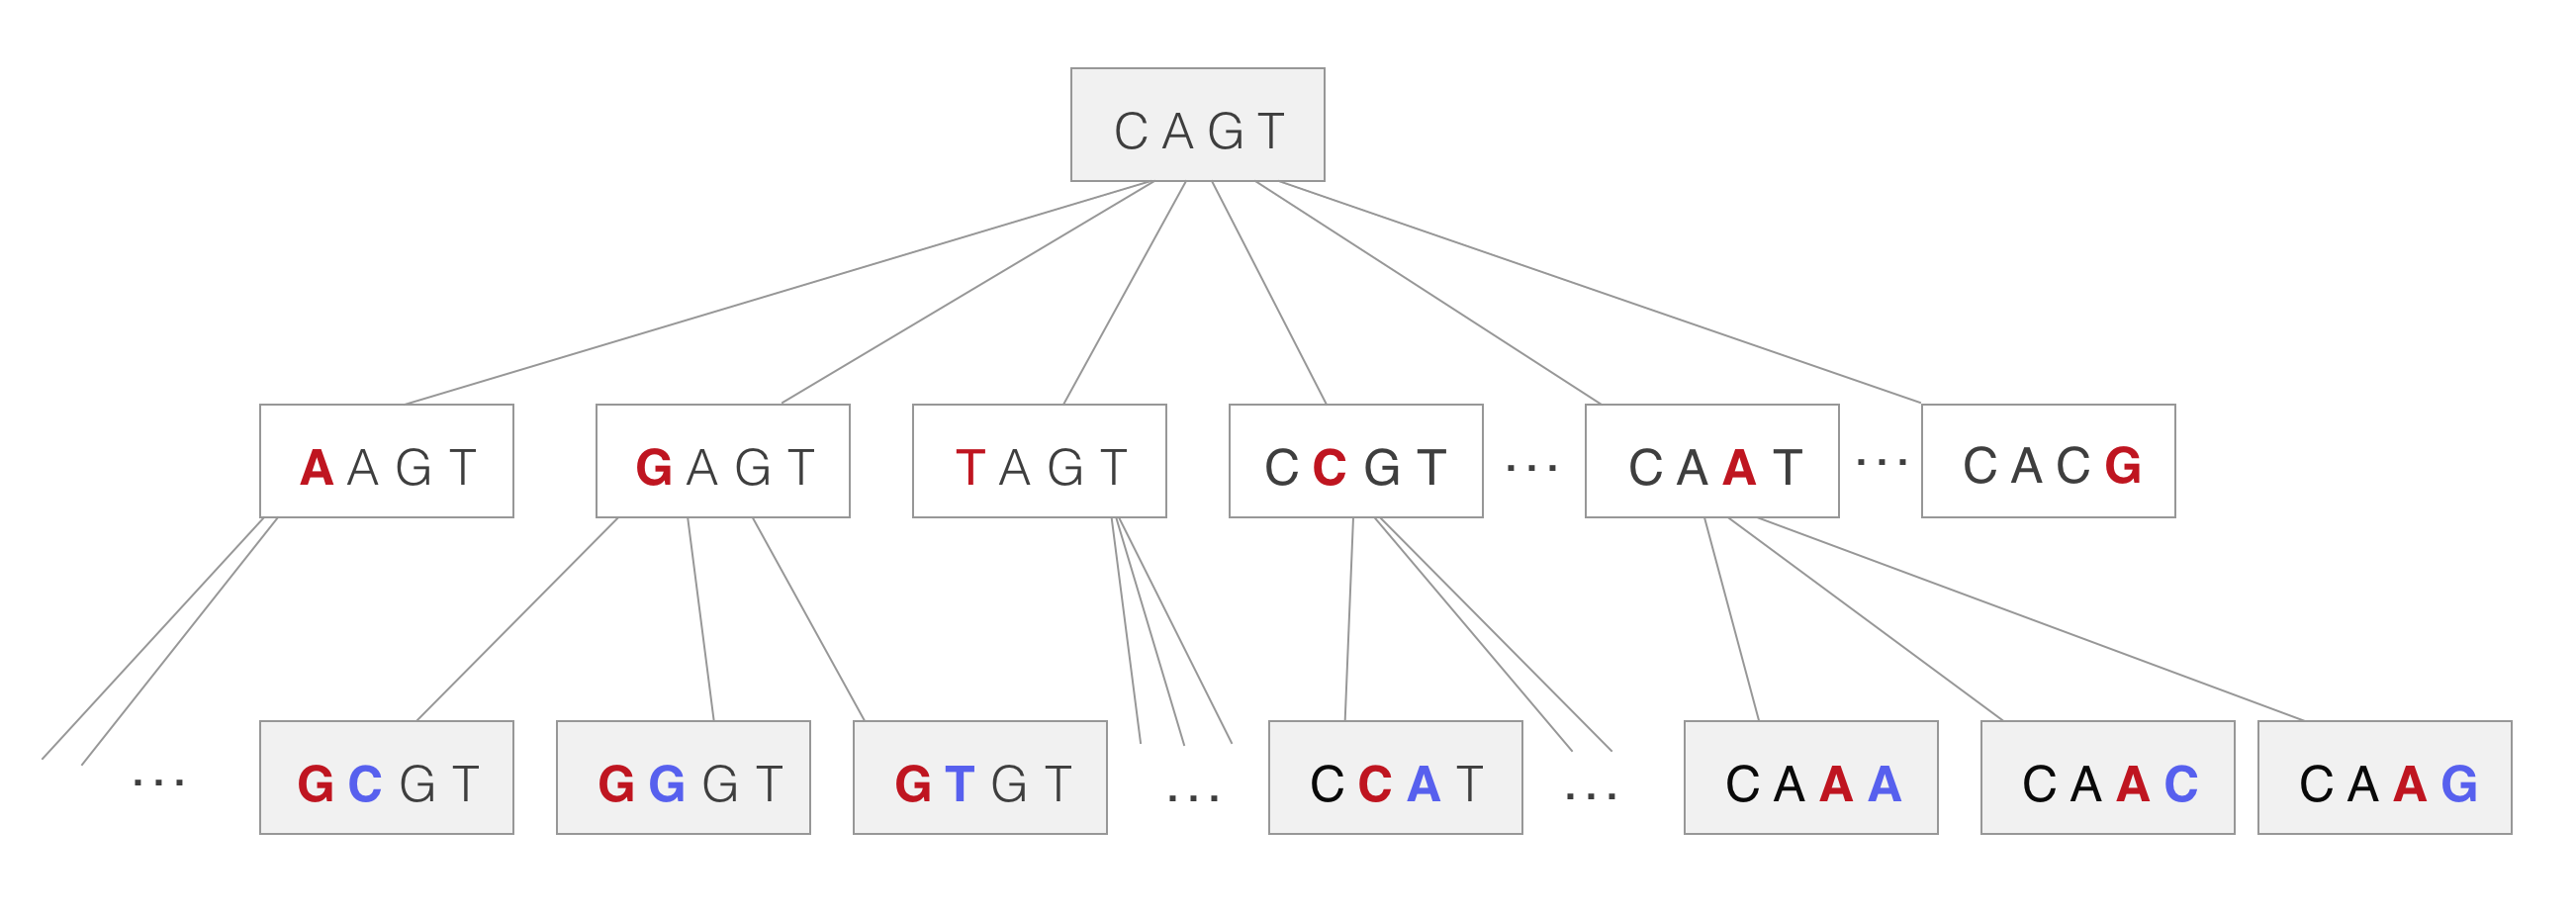
\includegraphics[width=5in]{contents/00_images/neighborhood-generation}\vspace*{5pt}
	\caption{Recursively generating the neighborhood of $l$-mer CACGT with $d = 2$}
	\label{fig:neighborhood-generation}
\end{figure}

	\subsubsection{Block-based optimization for neighborhood generation}
	The way EMS-GT represents the $d$-neighborhood $N_x$ of $l$-mer $x$ opens up a new way to improve the generation of neighborhood. $N_x$ is represented by a compresed $4^l$ bit flags array, where value of 1 corresponds to set membership, 0 if otherwise.  A previous study by Sia \cite{sia2015} improved the runtime performance in generating $N_x$. If $N_x$ is partitioned into blocks of $4^k$ bits each, where $k < l$, each block will conform into ($k$ + 2) bit patterns. By pre-computing these patterns, the algorithm can build the $N_x$ by blocks of bits instead of one bit at a time.

	\begin{figure}[h]
	\centering
	
\includegraphics[width=2.5in]{contents/00_images/0-1}\vspace*{5pt}
	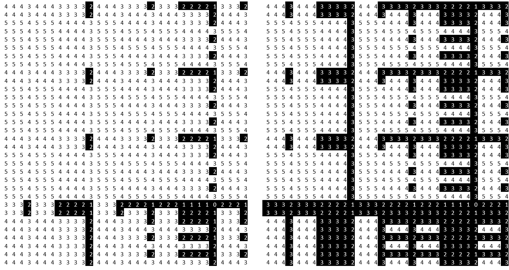
\includegraphics[width=2.5in]{contents/00_images/2-3}\vspace*{5pt}
	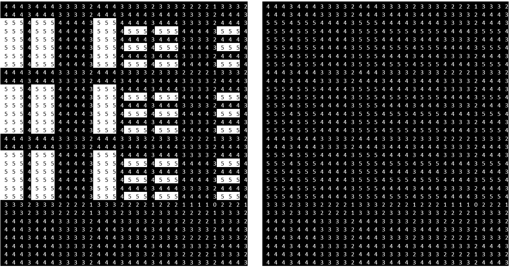
\includegraphics[width=2.5in]{contents/00_images/4-5}
	
	\caption{Bit patterns followed by blocks of size $4^{5}=32\times32$ in the bit-based representation of $\mathcal{N}(\texttt{acgtacgtacgt},5)$. Black signifies a 1. There are $(5+2)=7$ possible patterns---the empty pattern (all 0s) is not shown. Images from \cite{sia2015}}
	\label{fig:bit_patterns}
\end{figure}

	The algorithm divides the $l$-mer $x$ into its $(l - k)$-length prefix $y$ and suffix $z$ of length $k$. With the block patterns of $4^k$ $l$-mers generated, the algorithm recursively generates all possible prefix of $x$. For each prefix $y'$ generated, the algorithm applies the corresponding block pattern in $N_x$ based on $z$ and the remaining number of allowed mutations $d'$, where $d' = d - d_H(y, y')$. Specifically, EMS-GT builds the $\mathcal{N}_S$ using these steps:

	\begin{enumerate}
		\item Initialize $\mathcal{N}_S$ as an array of $4^l$ bits set to zero, and select a value for $k$.

		\item Pre-generate {\em Pattern}( $z$, $d_z$ ) for all $z \in \Sigma^k$ and all $d_z \in \{1,...,k-1\}$ to serve as bit masks for blocks. Note that block patterns for $d_z=0$ (one bit set) and $d_z=k$ (all bits set) will not require bit masks.

		\item For each $l$-mer $x = yz$ in sequence $S$: take each neighbor $y'$ of $y$, find the block in $\mathcal{N}_S$ whose prefix is $y'$, and compute the allowable suffix mismatches $d_z = d - d_H(y,y')$ within this block. Then,

			\begin{enumerate}
				\item if $d_z = 0$, set the bit at position $z$ in the block;
				\item if $d_z \geq k$, set all bits in the block to 1;
				\item otherwise, mask {\em Pattern}( $z$, $d_z$ ) onto the block.
			\end{enumerate}
	\end{enumerate}

	Choosing the optimum value for $k$ is important in this speedup technique. The $k$ value determines the runtime complexity of this technique since $k$ value determines the size of the block patterns. When $k$ value is higher, there are fewer prefix to generate recursively but each block bits setting is large. When $k$ value is lower, block bits setting is small but the algorithm has to recursively generate a larger number of prefix value of $l$-mer $x$. The optimum $k$ value used in the study is 5.

	
% {\setstretch{1.0} % Algorithm 4.1. Block Pattern Generation
\begin{figure}[h]
	\noindent \hspace*{6pt}{\bf Algorithm 2.1}
	\textsc{Block Pattern Generation}\small
	\begin{algorithmic}[1]\label{alg:block-pattern-gen}
		\Require block degree $k$
		\Ensure 3D bit-array $\mathcal{P}$ containing all possible non-trivial block patterns \vspace*{6pt}

		\State $\mathcal{P}[\ ][\ ][\ ] \leftarrow \{\}$ \hspace*{90pt}
		\Comment{retrieve a pattern $P$ as $\mathcal{P}[z][d - d_{y'}]$ }

		\For {$z \leftarrow 0$ to $4^k$}
		\For {$j \leftarrow 1$ to $k-1$}
		\For {$z' \leftarrow 0$ to $4^k$}
		\If{$dH(z,z') \leq j$} 
			\State $\mathcal{P}[z][j][z'] \leftarrow 1$
		\Else
			\State $\mathcal{P}[z][j][z'] \leftarrow 0$
		\EndIf\EndFor\EndFor\EndFor
		\State\Return $\mathcal{P}$
		\end{algorithmic}
\end{figure}



	% Elaborate and include results
	% Mention its competitiveness and a bit of introduction on possible areas of improvement 
	EMS-GT with this speedup technique has proven its competitiveness against algorithms qPMSPrune, qPMS7, PMS8 and qPMS9. Previous experimentations showed that EMS-GT with this speedup technique outperforms PMS8 in challenge instances (9, 2), (11, 3), (13, 4), (15, 5) and (17, 6). Compared to qPMS9, the improved EMS-GT is faster on all challenge instances mentioned except (17, 6). This study aims to outperform qPMS9 for challenges up to (17, 6).

	
\begin{figure}[ht]\label{fig:results2}
	\centering
	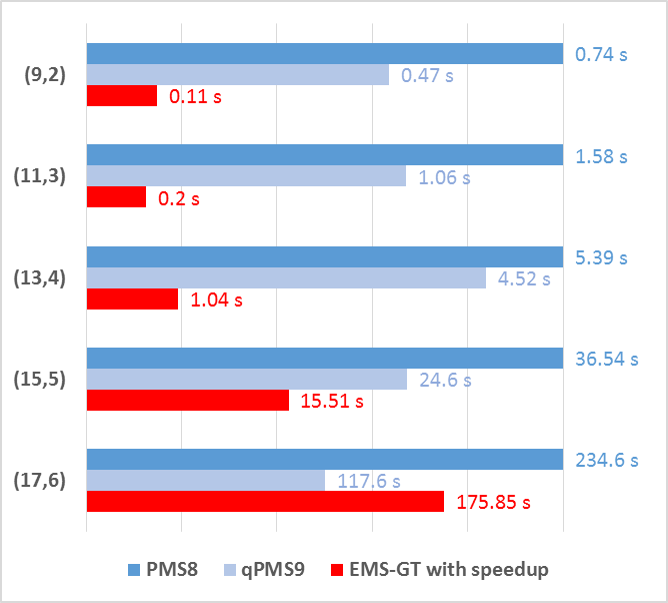
\includegraphics[width=4.0in]{contents/00_images/emsgt-with-speedup-vs-PMS,qPMS9}
	\caption{Improved EMS-GT's performance vs. PMS8 (baseline) and qPMS9. Images from \cite{sia2015}}
	\label{fig:sia-bar-results}
\end{figure}

% \begin{figure}[b]
	\noindent \hspace*{6pt}{\bf Algorithm 2} \textsc{Generate Neighborhood}
	\begin{algorithmic}[1]
		\label{alg:recursive-nbr-gen}
		\Require DNA sequence $S$, motif length $l$, mismatches $d$
		\Ensure bit-array $\mathcal{N}$ representing $\mathcal{N}(S,d)$ \vspace*{6pt}
		% \For{$i \leftarrow$ 1 to $4^{l}$}
		\State $\mathcal{N}[i] \leftarrow 0,\ \ \forall i < 4^{l}$ 
		% \EndFor
		\For{each $l$-mer $x$ in $S$}
			\State \textsc{AddNeighbors}($x$, 0, $d$) \hspace*{9pt}\Comment{recursive procedure}
		\EndFor
		\State \Comment{make $d$ changes in $l$-mer $x$, from position $s$ onward}
		\Procedure{AddNeighbors}{$x$, $s$, $d$}
			\For{$i \leftarrow s$ to $l$}
				\State $\Sigma \leftarrow$ \{\texttt{a}, \texttt{g}, \texttt{c}, \texttt{t}\} $- x_{i}$ \hspace*{6pt}\Comment{$i^{th}$ character in $x$}
				\For{$j \leftarrow 1$ to $|\Sigma|$}
					\State $neighbor \leftarrow\ ${\em\small concatenate}$(x_{1...i-1},\Sigma_{j},x_{i+1...l})$
					\State $\mathcal{N}[neighbor] \leftarrow 1$
					\If{$d > 1$ and $i < l$}
						\State \textsc{AddNeighbors}($neighbor$, $i+1$, $d-1$)
					\EndIf
				\EndFor
			\EndFor
		\EndProcedure
		\State\Return $\mathcal{N}$
	\end{algorithmic}
\end{figure}

Data structures and how an algorithm deals with the data commonly drive the performance of an algorithm. The EMS-GT algorithm uses a compressed bit-flag array for fast candidate motif elimination. Some key techniques that EMS-GT uses are defined in this section.

	\subsubsection{Integer mapping of $l$-mers}
	EMS-GT converts $l$-mers into its corresponding integer values. To achieve this, each character in the $l$-mer is translated using 2 bits (a=00, c=01, g=10, t=11). \newline
		{\small Ex.	\texttt{actg} maps to \texttt{00011110} and has an integer value of 30} 

	\subsubsection{Bit-based set representation and l-mer enumeration} 
	The EMS-GT maintains a $4^l$ array for enumerating all the possible $l$-mer values. The $l$-mer's integer value is used as the index value for the array. It uses the value of 1 if the $l$-mer is a member of the set, else it sets the value to 0.

	\subsubsection{Bit-array compression}
	To efficiently store these $l$-mers and save memory space, EMS-GT implements an approach that compresses the search space array using integer value bit flags. Instead of one $l$-mer per index value, the implementation can flag up to 32 $l$-mers (since we are using 32-bit integers) per index value. Figure \ref{fig:sample_search_space} shows a snapshot of the compressed bit array data structure. The explanation on how the algorithm accesses the bit flag is defined below: \newline

		{\small Ex. \texttt{gacgt} maps to \texttt{1000011011} = 539 in decimal.\newline
			\hspace*{64pt} \emph{bit position} = 539 mod 32 = 27;\newline
			\hspace*{64pt} \emph{array index}  = 539 / 32 = 16;\newline
			\hspace*{64pt} The bit flag for \texttt{gacgt} is in the 27$^{th}$ least significant bit\newline
			\hspace*{64pt} of the integer at array index 16.}

	\begin{figure}[t]
	\centering
	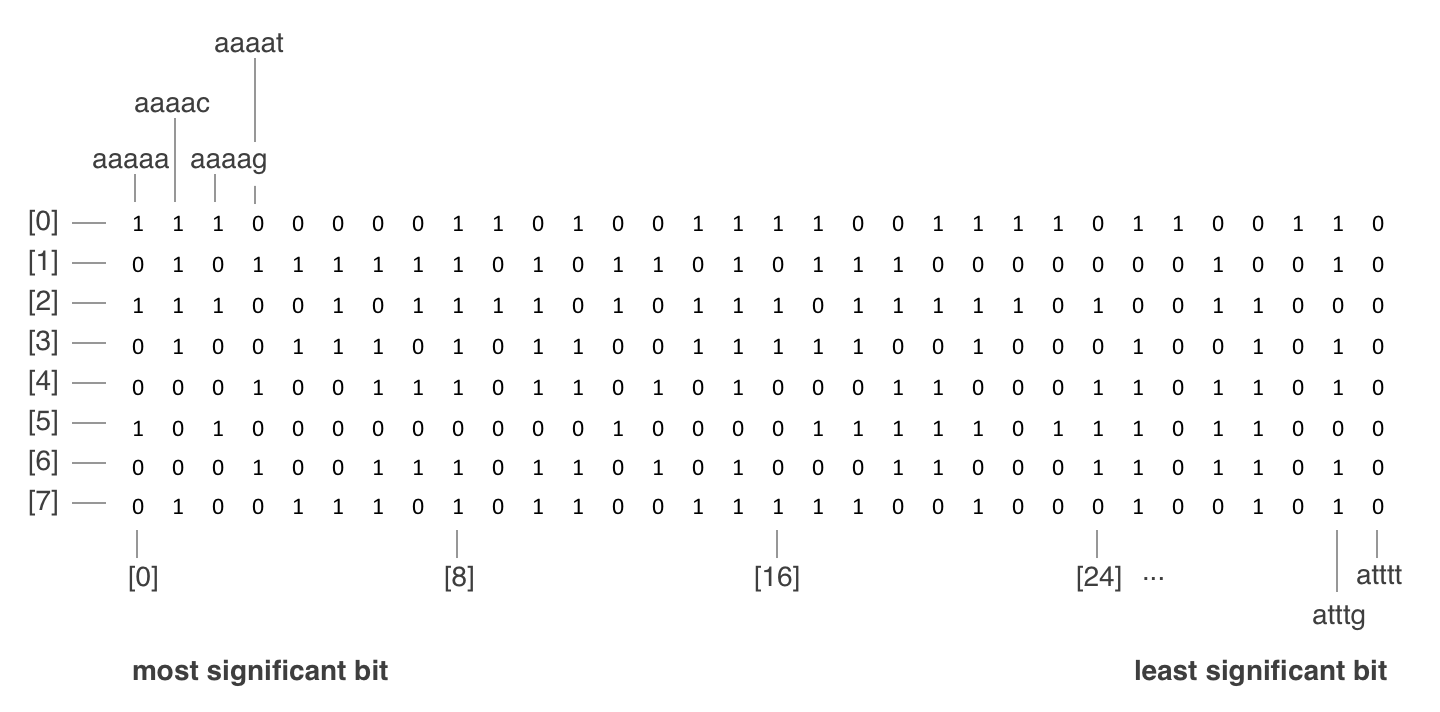
\includegraphics[width=5in]{contents/00_images/search_space}\vspace*{5pt}
	\caption{Example of $4^{5}$ search space showing its first 8 rows with random flag values.}
	\label{fig:sample_search_space}
\end{figure}

	\subsubsection{XOR-based Hamming distance computation}
	The mapping of an $l$-mer to its integer value has an additional advantage in computing for mismatch positions. Applying the boolean operator exclusive-or (XOR) between two integer values will return another integer value that contains nonzero value for mismatch positions. Counting this nonzero pairs of bits result to the hamming distance value. An example of this computation is shown below: \newline

	{\small Ex.	\texttt{aacgt} maps to \texttt{0000011011} \newline
		\vspace*{2pt}\hspace*{53pt} \underline{\texttt{tacgc} maps to \texttt{1100011001}} \newline
		\hspace*{55pt}	XOR produces \texttt{\uline{11}000000\uline{10}} = 2 mismatches.} \newline
		\hspace*{53pt} (Note, the mismatches are counted per pair)


	\subsubsection{Recursive neighborhood generation}
	The Generate phase of the algorithm produces the $d$-neighborhood of a string sequence by generating the $d$-neighborhood of all $l$-mers in that sequence. The implementation of EMS-GT uses a recursive approach for generating the $d$-neighborhood of an $l$-mer. The recursive generation can be visualized by a tree $\mathcal{T}(x)$ of height $d$ that is generated in depth-first manner. Each node is a tuple of $(w, p)$ where $w$ is an $l$-mer and $p$ corresponds to a position in the $l$-mer $0 \leq p \leq l$. At a given node $(w, p)$ and $p \neq l$, three children nodes are generated where each node is variant of $w$ that has a different character in $p + 1$ position. The root node is $(x, 0)$ and any $l$-mer in nodes at depth $t$ has a hamming distance of $t$ from the $l$-mer $x$. Figure \ref{fig:neighborhood-generation} illustrates the recursion tree of the neighborhood generation. Given this, the expected size of $N(x, d)$ can be computed using the equation: \newline
	\begin{equation}
		|N(x,d)| = \sum_{i=0}^d \binom{l}{i} 3^{i}
	\end{equation}

	\begin{figure}[h]
	\centering
	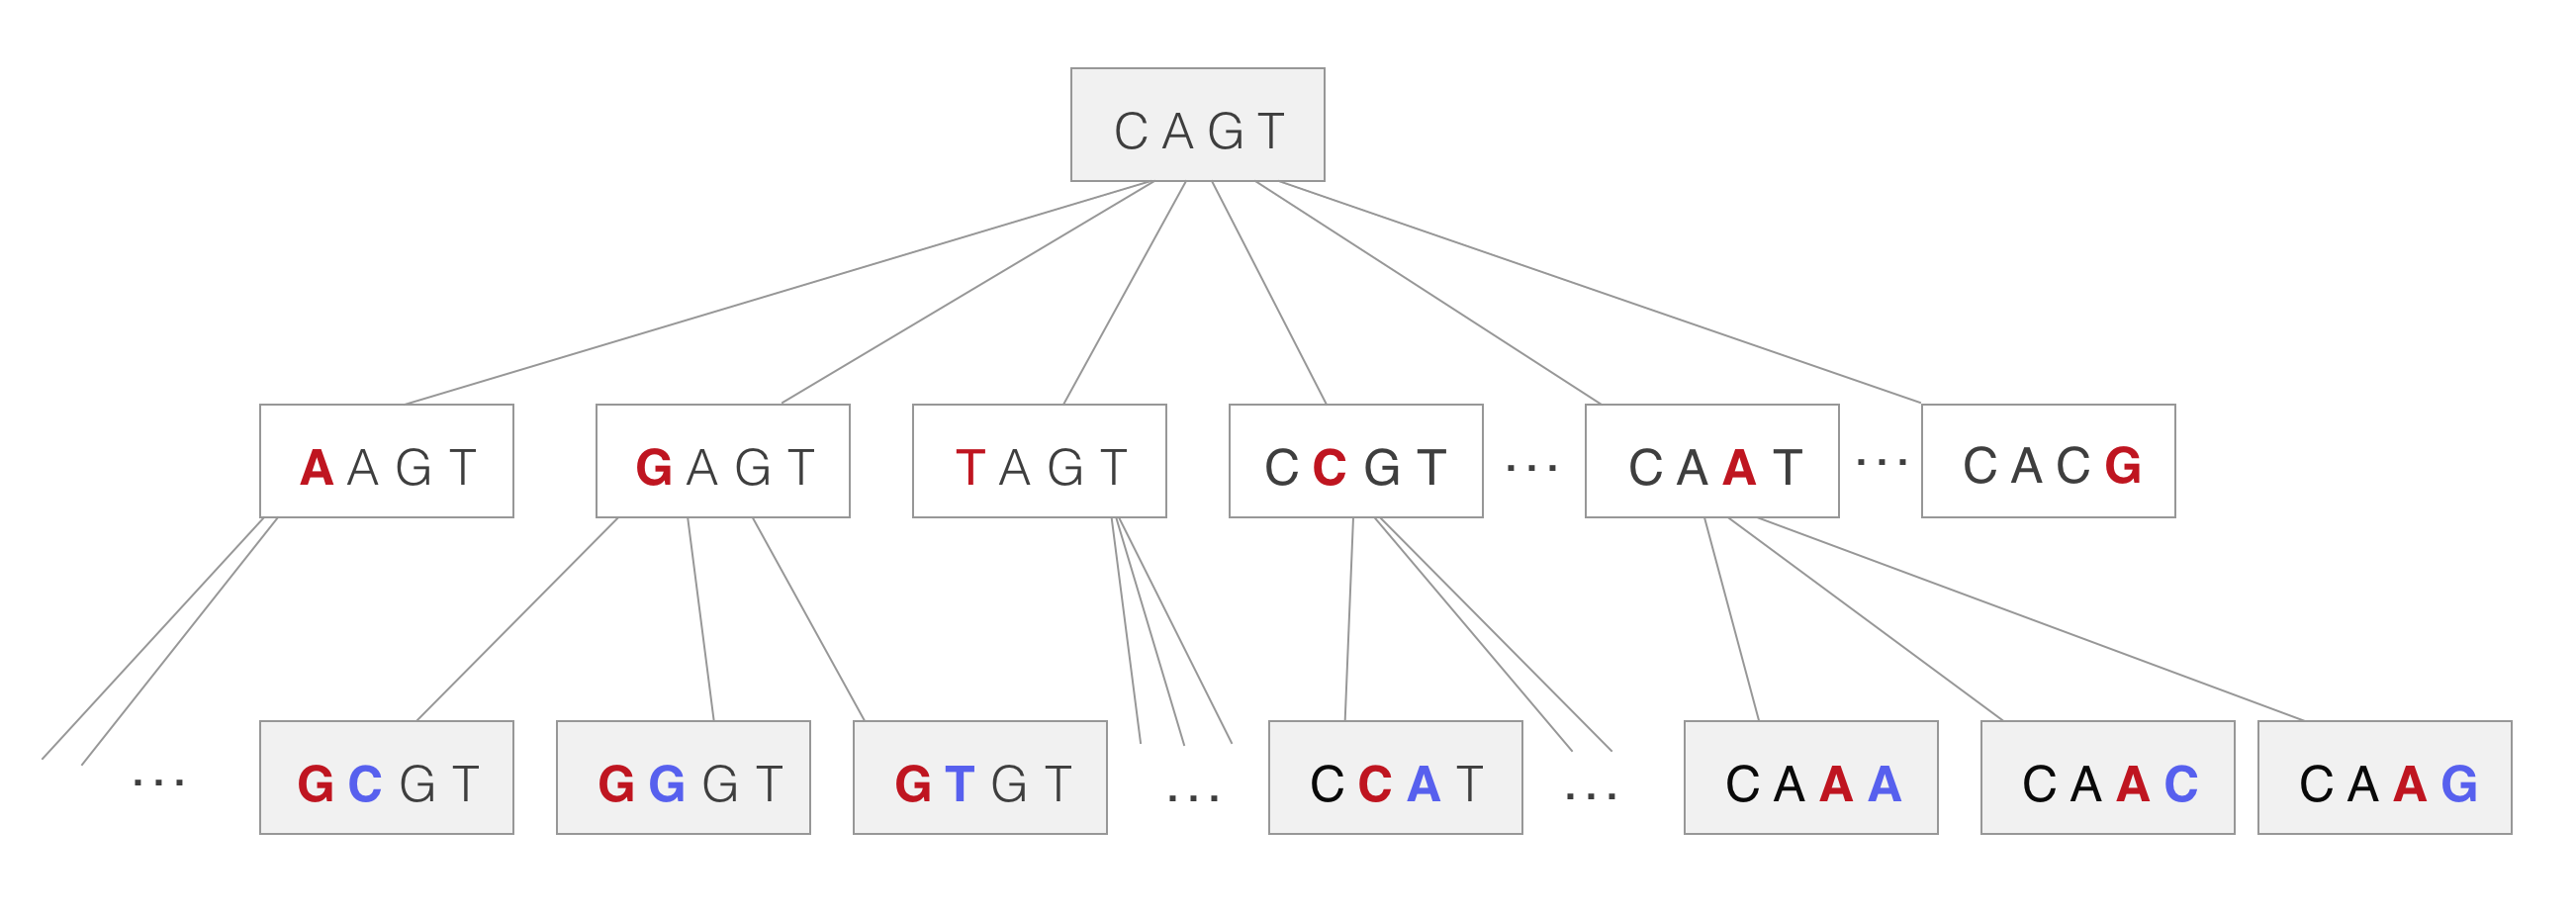
\includegraphics[width=5in]{contents/00_images/neighborhood-generation}\vspace*{5pt}
	\caption{Recursively generating the neighborhood of $l$-mer CACGT with $d = 2$}
	\label{fig:neighborhood-generation}
\end{figure}

	\subsubsection{Block-based optimization for neighborhood generation}
	The way EMS-GT represents the $d$-neighborhood $N_x$ of $l$-mer $x$ opens up a new way to improve the generation of neighborhood. $N_x$ is represented by a compresed $4^l$ bit flags array, where value of 1 corresponds to set membership, 0 if otherwise.  A previous study by Sia \cite{sia2015} improved the runtime performance in generating $N_x$. If $N_x$ is partitioned into blocks of $4^k$ bits each, where $k < l$, each block will conform into ($k$ + 2) bit patterns. By pre-computing these patterns, the algorithm can build the $N_x$ by blocks of bits instead of one bit at a time.

	\begin{figure}[h]
	\centering
	
\includegraphics[width=2.5in]{contents/00_images/0-1}\vspace*{5pt}
	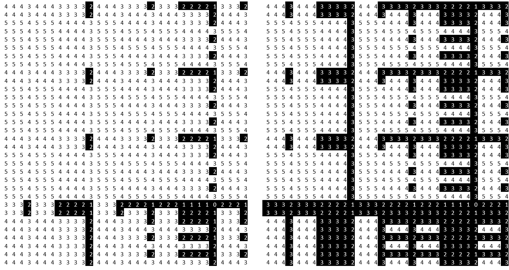
\includegraphics[width=2.5in]{contents/00_images/2-3}\vspace*{5pt}
	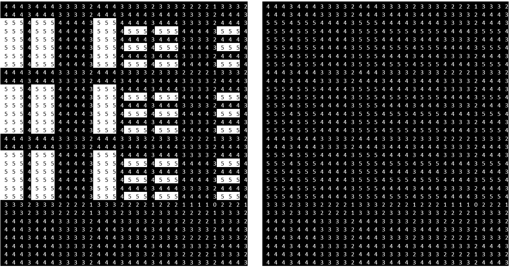
\includegraphics[width=2.5in]{contents/00_images/4-5}
	
	\caption{Bit patterns followed by blocks of size $4^{5}=32\times32$ in the bit-based representation of $\mathcal{N}(\texttt{acgtacgtacgt},5)$. Black signifies a 1. There are $(5+2)=7$ possible patterns---the empty pattern (all 0s) is not shown. Images from \cite{sia2015}}
	\label{fig:bit_patterns}
\end{figure}

	The speedup-technique divides the $l$-mer $x$ into its $(l - k)$-length prefix $y$ and suffix $z$ of length $k$. With the block patterns of $4^k$ $l$-mers generated, the algorithm recursively generates all possible prefix of $x$. For each prefix $y'$ generated, the algorithm applies the corresponding block pattern in $N_x$ based on $z$ and the remaining number of allowed mutations $d'$, where $d' = d - d_H(y, y')$. As defined in the study, EMS-GT builds the $\mathcal{N}_S$ using these steps:

	\begin{enumerate}
		\item Initialize $\mathcal{N}_S$ as an array of $4^l$ bits set to zero, and select a value for $k$.

		\item Pre-generate {\em Pattern}( $z$, $d_z$ ) for all $z \in \Sigma^k$ and all $d_z \in \{1,...,k-1\}$ to serve as bit masks for blocks. Note that block patterns for $d_z=0$ (one bit set) and $d_z=k$ (all bits set) will not require bit masks.

		\item For each $l$-mer $x = yz$ in sequence $S$: take each neighbor $y'$ of $y$, find the block in $\mathcal{N}_S$ whose prefix is $y'$, and compute the allowable suffix mismatches $d_z = d - d_H(y,y')$ within this block. Then,

			\begin{enumerate}
				\item if $d_z = 0$, set the bit at position $z$ in the block;
				\item if $d_z \geq k$, set all bits in the block to 1;
				\item otherwise, mask {\em Pattern}( $z$, $d_z$ ) onto the block.
			\end{enumerate}
	\end{enumerate}

	Choosing the optimum value for $k$ is important in this speedup technique. The $k$ value determines the runtime complexity of this technique since $k$ value determines the size of the block patterns. When $k$ value is higher, there are fewer prefix to generate recursively but each block bits setting is large. When $k$ value is lower, block bits setting is small but the algorithm has to recursively generate a larger number of prefix value of $l$-mer $x$. The optimum $k$ value used in the study is 5.

	
% {\setstretch{1.0} % Algorithm 4.1. Block Pattern Generation
\begin{figure}[h]
	\noindent \hspace*{6pt}{\bf Algorithm 2.1}
	\textsc{Block Pattern Generation}\small
	\begin{algorithmic}[1]\label{alg:block-pattern-gen}
		\Require block degree $k$
		\Ensure 3D bit-array $\mathcal{P}$ containing all possible non-trivial block patterns \vspace*{6pt}

		\State $\mathcal{P}[\ ][\ ][\ ] \leftarrow \{\}$ \hspace*{90pt}
		\Comment{retrieve a pattern $P$ as $\mathcal{P}[z][d - d_{y'}]$ }

		\For {$z \leftarrow 0$ to $4^k$}
		\For {$j \leftarrow 1$ to $k-1$}
		\For {$z' \leftarrow 0$ to $4^k$}
		\If{$dH(z,z') \leq j$} 
			\State $\mathcal{P}[z][j][z'] \leftarrow 1$
		\Else
			\State $\mathcal{P}[z][j][z'] \leftarrow 0$
		\EndIf\EndFor\EndFor\EndFor
		\State\Return $\mathcal{P}$
		\end{algorithmic}
\end{figure}



	
\begin{figure}[ht]\label{fig:results2}
	\centering
	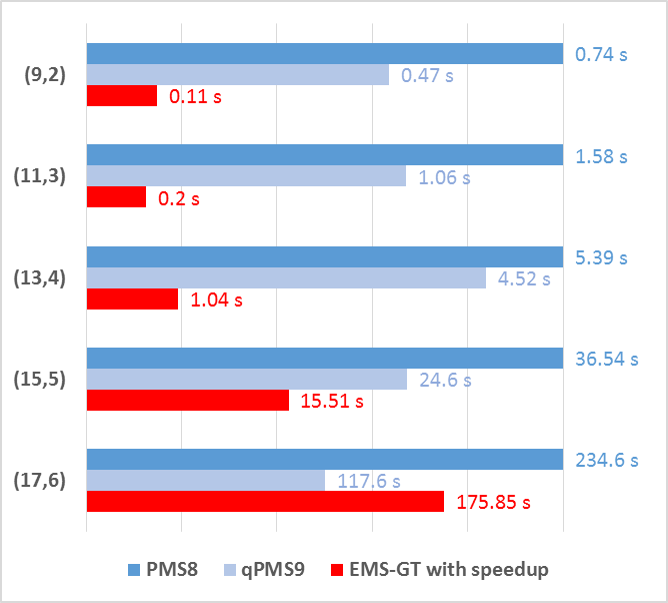
\includegraphics[width=4.0in]{contents/00_images/emsgt-with-speedup-vs-PMS,qPMS9}
	\caption{Improved EMS-GT's performance vs. PMS8 (baseline) and qPMS9. Images from \cite{sia2015}}
	\label{fig:sia-bar-results}
\end{figure}
	
	% Elaborate and include results
	% Mention its competitiveness and a bit of introduction on possible areas of improvement 
	EMS-GT with this speedup technique has proven its competitiveness against algorithms qPMSPrune, qPMS7, PMS8 and qPMS9. Previous experimentations showed that EMS-GT with this speedup technique outperforms PMS8 in challenge instances (9, 2), (11, 3), (13, 4), (15, 5) and (17, 6). Compared to qPMS9, the improved EMS-GT is faster on all challenge instances mentioned except (17, 6). This study aims to improve the EMS-GT algorithm so that it outperforms qPMS9 for challenges up to (17, 6).

